% !TEX TS-program = pdflatex
% !TEX encoding = UTF-8 Unicode

% Matthew Urffer Master Thesis
% 
% Pulse Shape Discrimination
%
\section{Pulse Shape Discrimination}

%%%%%%%%%%%%%%%%%%%%%%%%%%%%%%%%%%%%%%%%%%%%%%%%%%%%%%%%%%%%%%%%%%%%%%%%%%%%%%%
%                                                                             %
%                                    METHODS                                  %
%                                                                             %
%%%%%%%%%%%%%%%%%%%%%%%%%%%%%%%%%%%%%%%%%%%%%%%%%%%%%%%%%%%%%%%%%%%%%%%%%%%%%%%

\subsection{PSD Introduction}
%%%%%%%%%%%%%%%%%%%%%%%%%%%%%%%%%%%%%%%%%%%%%%%%%%%%%%%%%%%%%%%%%%%%%%%%%%%%%%%
\begin{frame}{Introduction to PSD}
	\begin{itemize}
		\small
		\item Determination of incident radation from pulse shape
		\item Physical basis
		\begin{itemize}
			\tiny
			\item Difference in singlet ($S_1$) and triplet ($T_1$) states \cite{zaitseva_plastic_2012}
			\item Triple states annihilate: $T_1 + T_1 \to S_0 + S_1$
			\item Product states have a longer and delayed time scale
		\end{itemize}
		\small
		\item Short range of energetic protons (neutron interactions) cause a high concentration of triplet states than from electrons from gamma
		\item Lots of methods exist \cite{ambers_hybrid_2011, gamage_comparison_2011, miller_digital_2007}
		\begin{itemize}
			\tiny
			\item Charge Integration
			\item Pulse Gradient Analysis
			\item Neutron-$\gamma$ Modal Analysis
			\item Pulse Shape Parameters
			\item Artifical Neural Networks
			\item and more!
		\end{itemize}
	\end{itemize}
\end{frame}
%%%%%%%%%%%%%%%%%%%%%%%%%%%%%%%%%%%%%%%%%%%%%%%%%%%%%%%%%%%%%%%%%%%%%%%%%%%%%%%
\begin{frame}{PSD Methods}
\begin{columns}[onlytextwidth]
\begin{column}{0.45\textwidth}
	Alpha are used as surrogate neutrons
	\newtheorem{thm9}{Charge Ratio Method}
	\begin{thm9}<1->
		$$ R_C = \frac{\int_{X_0}^{\infty}{f(x)dx}}{\int_{0}^{\infty}{f(x)dx}} $$
	where:
	\begin{itemize}
		\tiny
		\item $R_C$ is the charge ratio
		\item $f(x)$ is the spectra
		\item $\int_{X_0}^{\infty}{f(x)dx}$ slow charge
		\item $\int_{0}^{\infty}{f(x)dx}$ fast charge
	\end{itemize}
	\end{thm9}
\end{column}
\begin{column}{0.45\textwidth}
	\begin{figure}
		\centering
		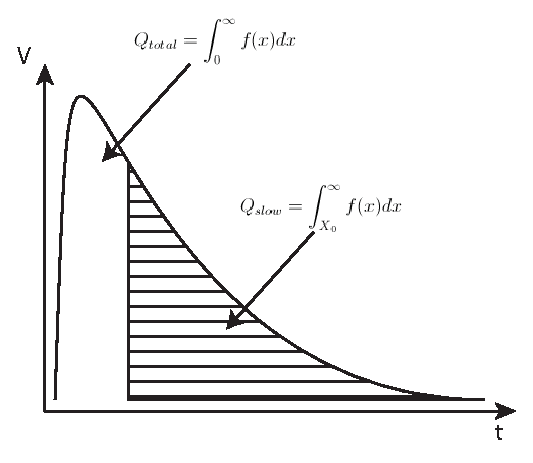
\includegraphics[height=0.5\textwidth]{images/PSD_Spectra.eps}
		\caption{Charge Ratio Method}
		\label{fig:PSD_ChargeRatio}
	\end{figure}
\end{column}
\end{columns}

	\begin{itemize}
		\tiny
		\item MLLD for a film is determined from a ${}^{60}$Co measurement
		\item Source produces a 10 mR/hr field at detector surface
		\item Particles incident determined from simulation
	\end{itemize}
\end{frame}
%%%%%%%%%%%%%%%%%%%%%%%%%%%%%%%%%%%%%%%%%%%%%%%%%%%%%%%%%%%%%%%%%%%%%%%%%%%%%%%
\begin{frame}{ROC Curves}
	\begin{table}[h]
	\begin{tabular}{m{1cm} | m{1.5cm}| >{\centering\arraybackslash}m{2cm} >{\centering\arraybackslash}m{2cm}}
	\tiny
		 & \multicolumn{3}{c}{True Class} \\
		 \hline
		 \hline
		 \multirow{3}{*}{\protect \begin{sideways} Hypothesized Class \protect \end{sideways}} & & Alpha & Gamma \\  \cdashline{3-4}
		 & Alpha & True Postive & False Postive (Type 1) \\ \cdashline{3-4}
		 & Gamma & False Negative (Type 2) & True Negative \\ 
	\end{tabular}
	\end{table}
	\begin{figure}
		\centering
		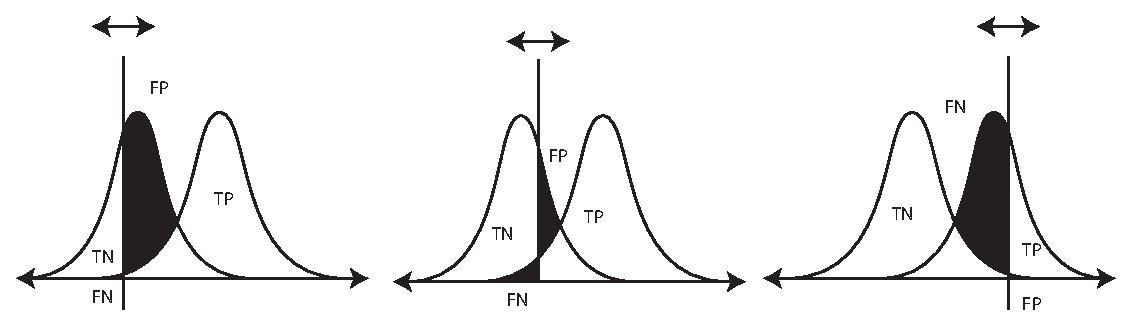
\includegraphics[height=0.4\textheight]{images/ROC_Diagrams.eps}
		\caption{Perforamnce of a Classifier}
		\label{fig:ROCDiagrams}
	\end{figure}
\end{frame}
%%%%%%%%%%%%%%%%%%%%%%%%%%%%%%%%%%%%%%%%%%%%%%%%%%%%%%%%%%%%%%%%%%%%%%%%%%%%%%%
